%!TEX root = main.tex

\chapter{Theory}
\section{Starcraft}

\begin{figure}[h!tb]
\centering
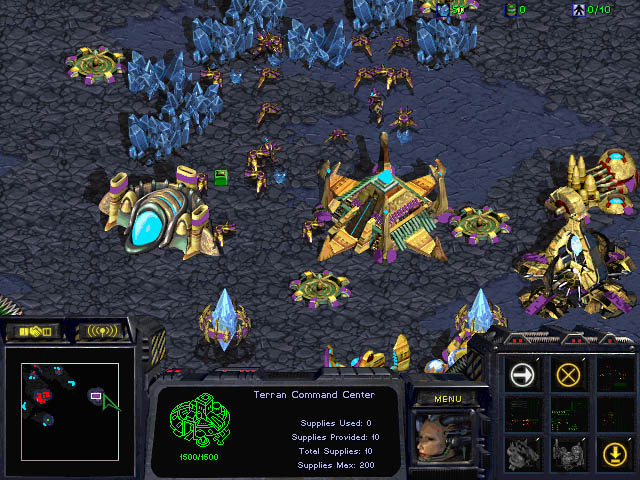
\includegraphics[scale=0.5]{graphics/scbw.jpg}
\caption{Star Craft Brood War}
\label{fig:scbwIntro}
\end{figure}
StarCraft is on the surface a very simple game, it has only three different playable races, a
handful of different buildings and units, and relatively simple to comprehend
goals. But once you start analyzing the game, the reality is quite different. The brood war expansion pack was released back in 1998, and has been played at a high level since that and all the way up to today. And the meta game has evolved during the entire lifespan of the game and is still changing today with new tactics showing up from tournament to tournament.
\cite{blizzardstarcraft}

When playing at a really high level you are working with really small windows of opportunity, often called timings. And it is these timings that enable a game with what should in theory be simple elements to have such complex and evolving strategies. 


\section{Artificial Intelligences for StarCraft}
There have been a handful of relatively successful AIs for StarCraft.

\subsection{In-game AI}
The in-game AI is considered not very good.

\subsection{Berkeley Overmind}
This is considered one of the best AIs, not perhaps because it is very complex,
but because it has a solid ``cheese'' and has been well-tweaked.


\section{Architectures}
\subsection{General architectures}
\subsubsection{}
\subsection{Cognitive Architectures}
\paragraph{Global Workspace Theory}
\paragraph{Cognitive Models in game AIs}
\cite{Arrabales2009}
